% !TeX root = ../main.tex
\section{Evidence-Linked Choreography Supervision}
\label{sec:data}
% !TeX root = ../main.tex
\begin{figure*}[t]
\centering
\begin{subfigure}{\textwidth}
\centering
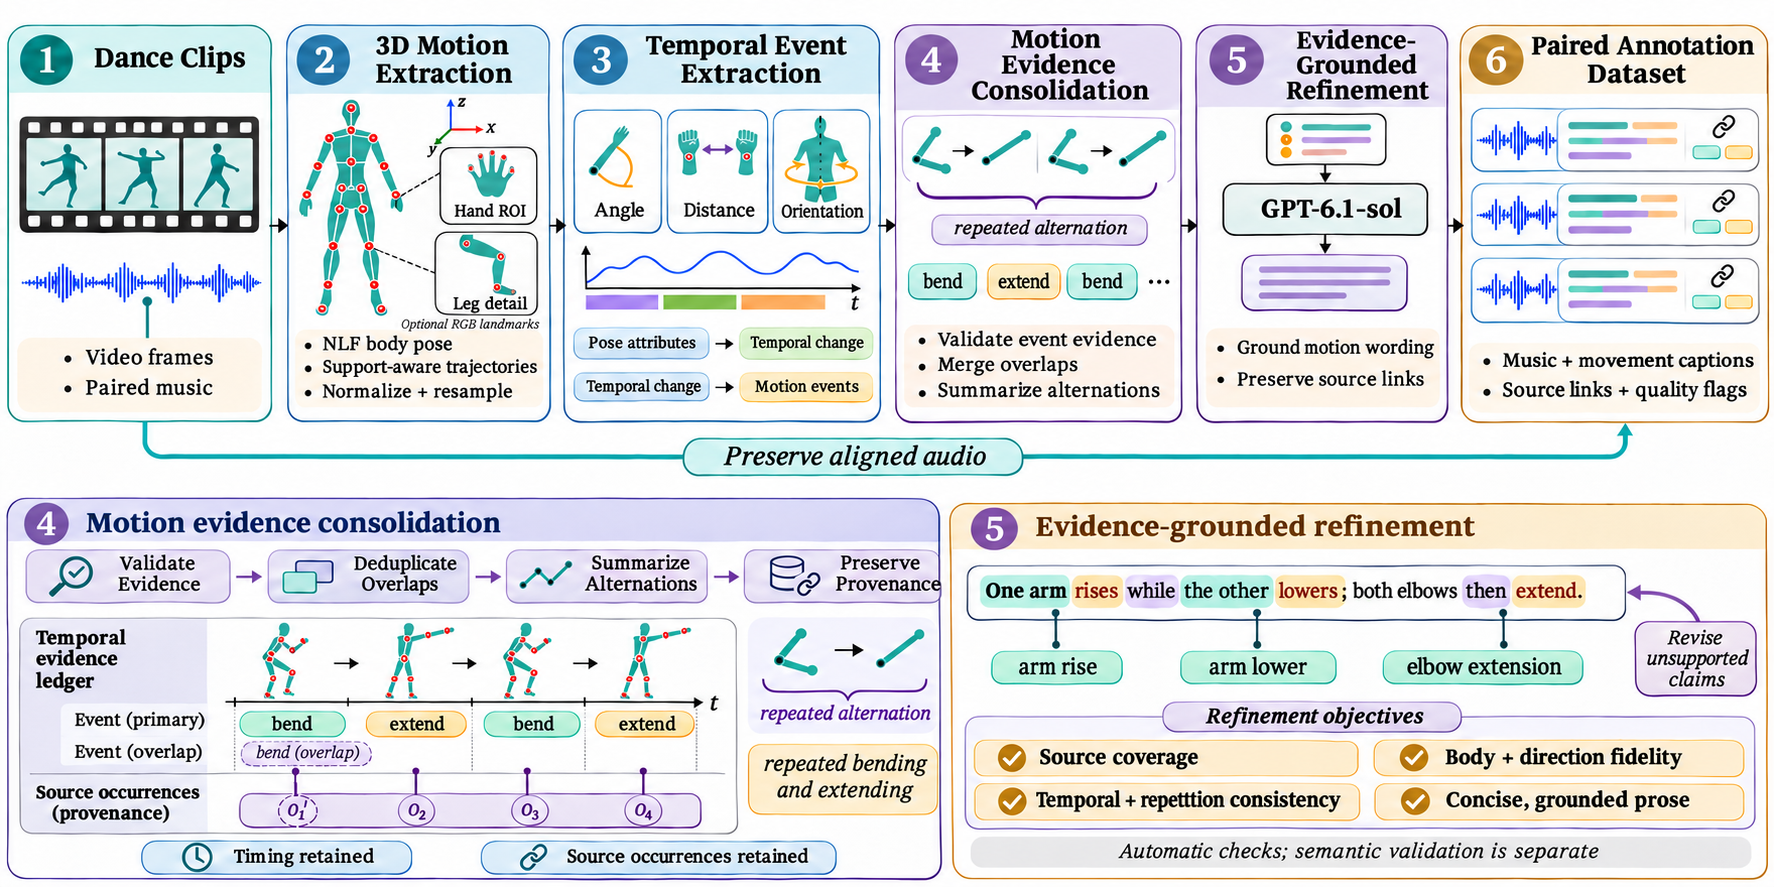
\includegraphics[width=\textwidth]{figures/annotation_pipeline_v5.png}
\caption{Geometry-based annotation framework and evidence-preserving refinement.}
\label{fig:annotation-pipeline}
\end{subfigure}
\par\medskip
\begin{subfigure}{\textwidth}
\centering
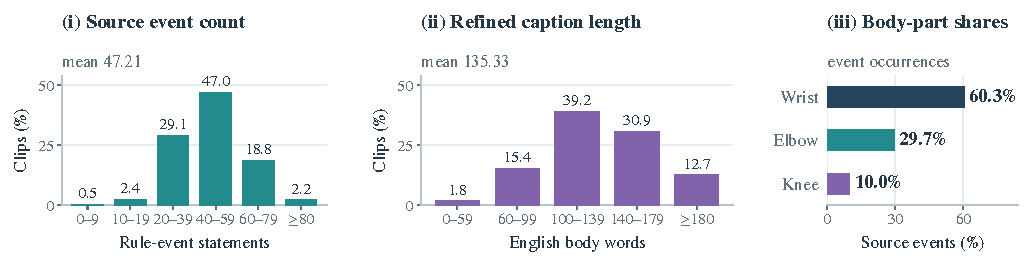
\includegraphics[width=\textwidth]{figures/annotation_distributions_v3.pdf}
\caption{Descriptive statistics on the same 22,352 paired clips.}
\label{fig:annotation-distributions}
\end{subfigure}
\caption{\textbf{Annotation construction and supervision profile.}
(a) MotionScript-based temporal extraction~\cite{motionscript},
Motion Evidence Consolidation, and GPT-6.1-sol evidence-grounded
refinement retain source occurrences and paired music. Hand/leg insets
are detail views; matching 4/5 badges identify expanded stages.
This is a component-integration framework; current experimental labels
come from the existing 2D rule-log rewrite route, detailed in
Appendix~\ref{sec:annotation-details}.
(b) Frozen paired statistics retain all automatic quality flags.
Event occurrences, caption body words, and body-part shares use different
units; they characterize supervision rather than gains in action accuracy
or diversity. The style prefix is excluded from word counts.}
\label{fig:dataset-overview}
\end{figure*}


\paragraph{Paired resource.}
The collection contains 220,667 music--choreography records, partitioned
into 198,315 training, 11,098 validation, and 11,254 test records.
Records retain media identity, observation intervals, source groups,
and annotation metadata. These inventory counts do not establish the
model's exact training subset without its training manifest; video-source
grouping likewise does not establish song-level disjointness.

\paragraph{From movement evidence to language.}
Current references are GPT-6.1-sol text-only rewrites of windowed 2D
rule-event logs: sixteen event types describe wrist directions and
projected elbow/knee angle changes. \emph{Evidence-Grounded Refinement}
targets source coverage, body/direction fidelity, timing/repetition
consistency, and concise grounded prose. Sentences link to source-event
IDs; automatic flags support auditing without human semantic approval.
The refiner receives no audio; aligned music is retained for subsequent
learning. Open-vocabulary prose remains bounded by observed events.
Figure~\ref{fig:choreography-example} illustrates how a score states body
references, movement range, and order, then carries an explicit end state
into the next action. Its author-composed instructions accompany real media.
% !TeX root = ../main.tex
\begin{figure*}[t]
\centering
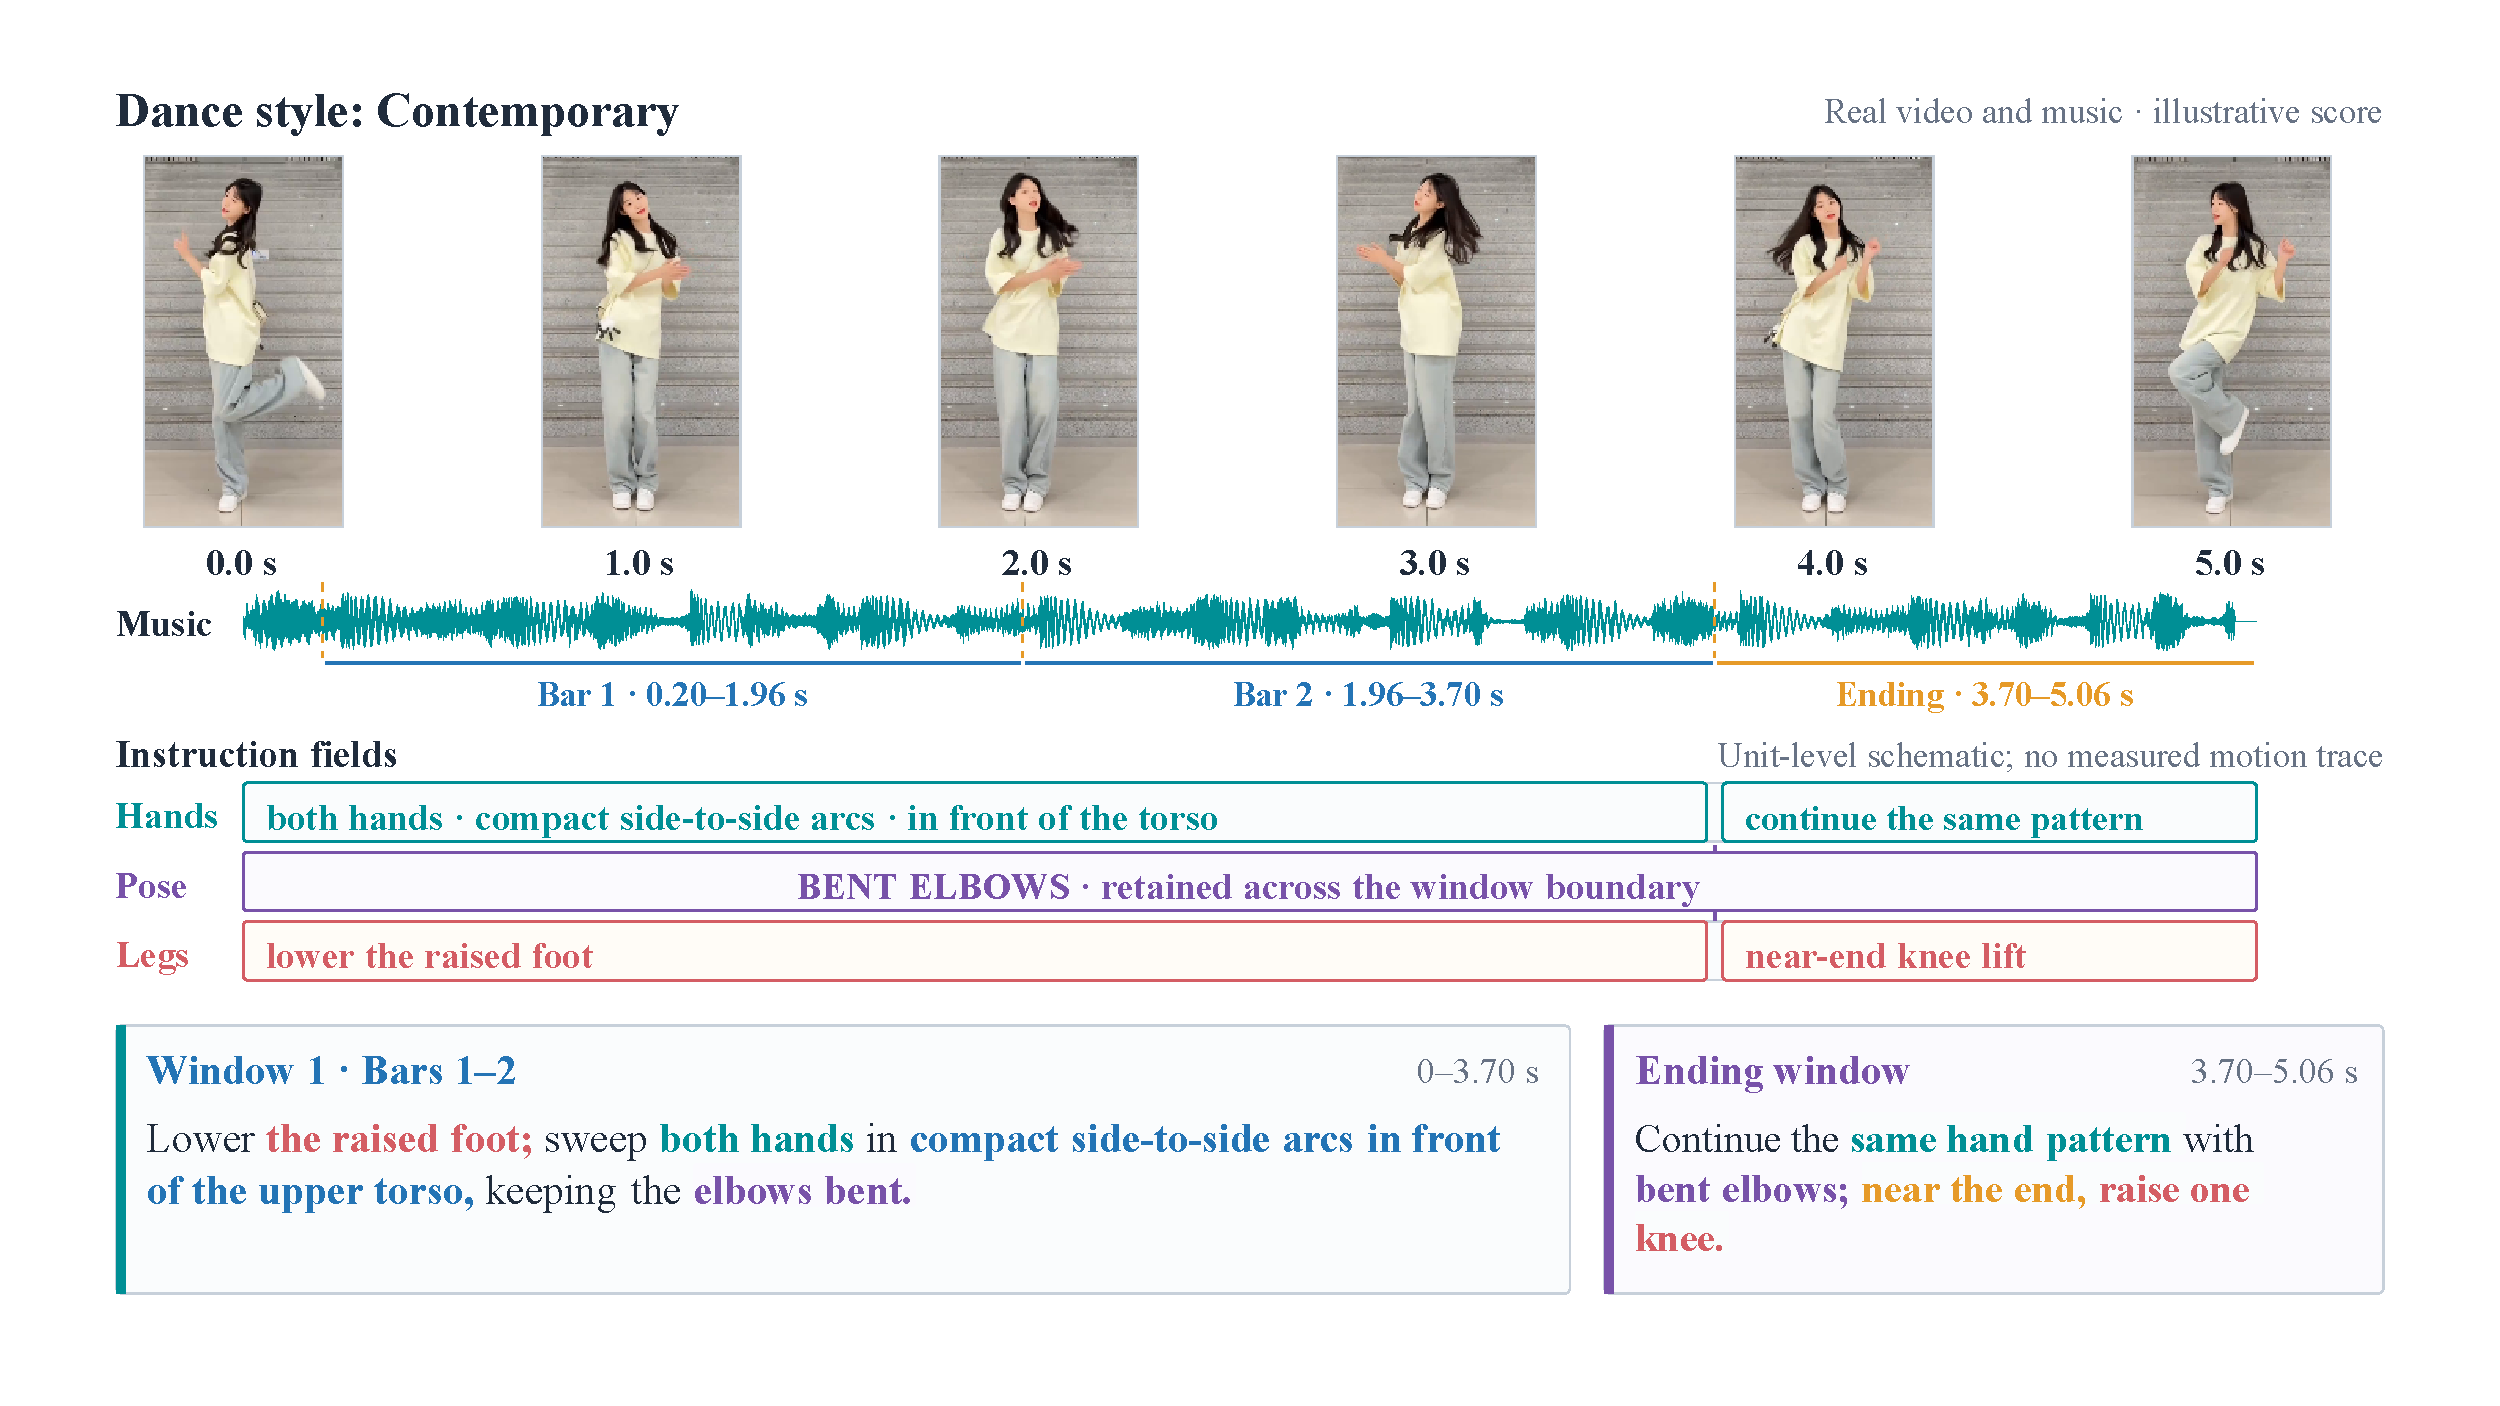
\includegraphics[width=\textwidth]{figures/revision_20261117_v3/paper/choreography_case.pdf}
\caption{\textbf{What makes a movement description informative.}
Six equally spaced real frames share a clock with the measured music
waveform. Unit-level fields expose body references, movement range and
direction, and the retained elbow state; matching colors connect these
fields to the instructions below. Predicted bars form a two-bar unit and
an ending fragment, with the initial 0--0.20\,s fragment merged.
The authored instructions and field bands illustrate the representation,
not scored predictions, measured action durations, or verified synchronization.}
\label{fig:choreography-example}
\end{figure*}


\paragraph{Geometry and evidence consolidation.}
Figure~\ref{fig:annotation-pipeline} depicts the geometry extension using
NLF~\cite{nlf} and MotionScript~\cite{motionscript}. Body-relative signals
are resampled to 20~FPS; support masks preserve unsupported intervals.
\emph{Motion Evidence Consolidation} validates evidence, deduplicates
overlaps, summarizes supported alternations, and preserves source
occurrences. Optional direct-RGB palm/foot landmarks and DWPose hand
observations supplement body geometry; template joints add no observation.
Hand insets magnify keypoints, rather than denote an implemented
independent ROI estimator. This 3D route is not established as the
production source of current labels. Appendix~\ref{sec:annotation-details}
details provenance.

\paragraph{Descriptive statistics.}
Figure~\ref{fig:annotation-distributions} compares the same 22,352 paired
validation/test clips, retaining all quality flags. Source-style metadata
are unchanged and unknown for 59.6\%. Event and word counts have
different units and do not establish greater action diversity.
References describe individual observed dances; agreement does not
imply a unique choreography for the music.
